%---------------------------------------------------------
%	6. DEMO & IMPACT
%---------------------------------------------------------
\section{Demo}

\begin{frame}
    \frametitle{Product Demo: NightClear Web App}
    \framesubtitle{Web application built with Gradio}

    \begin{columns}[c]
        \begin{column}{0.62\textwidth}
            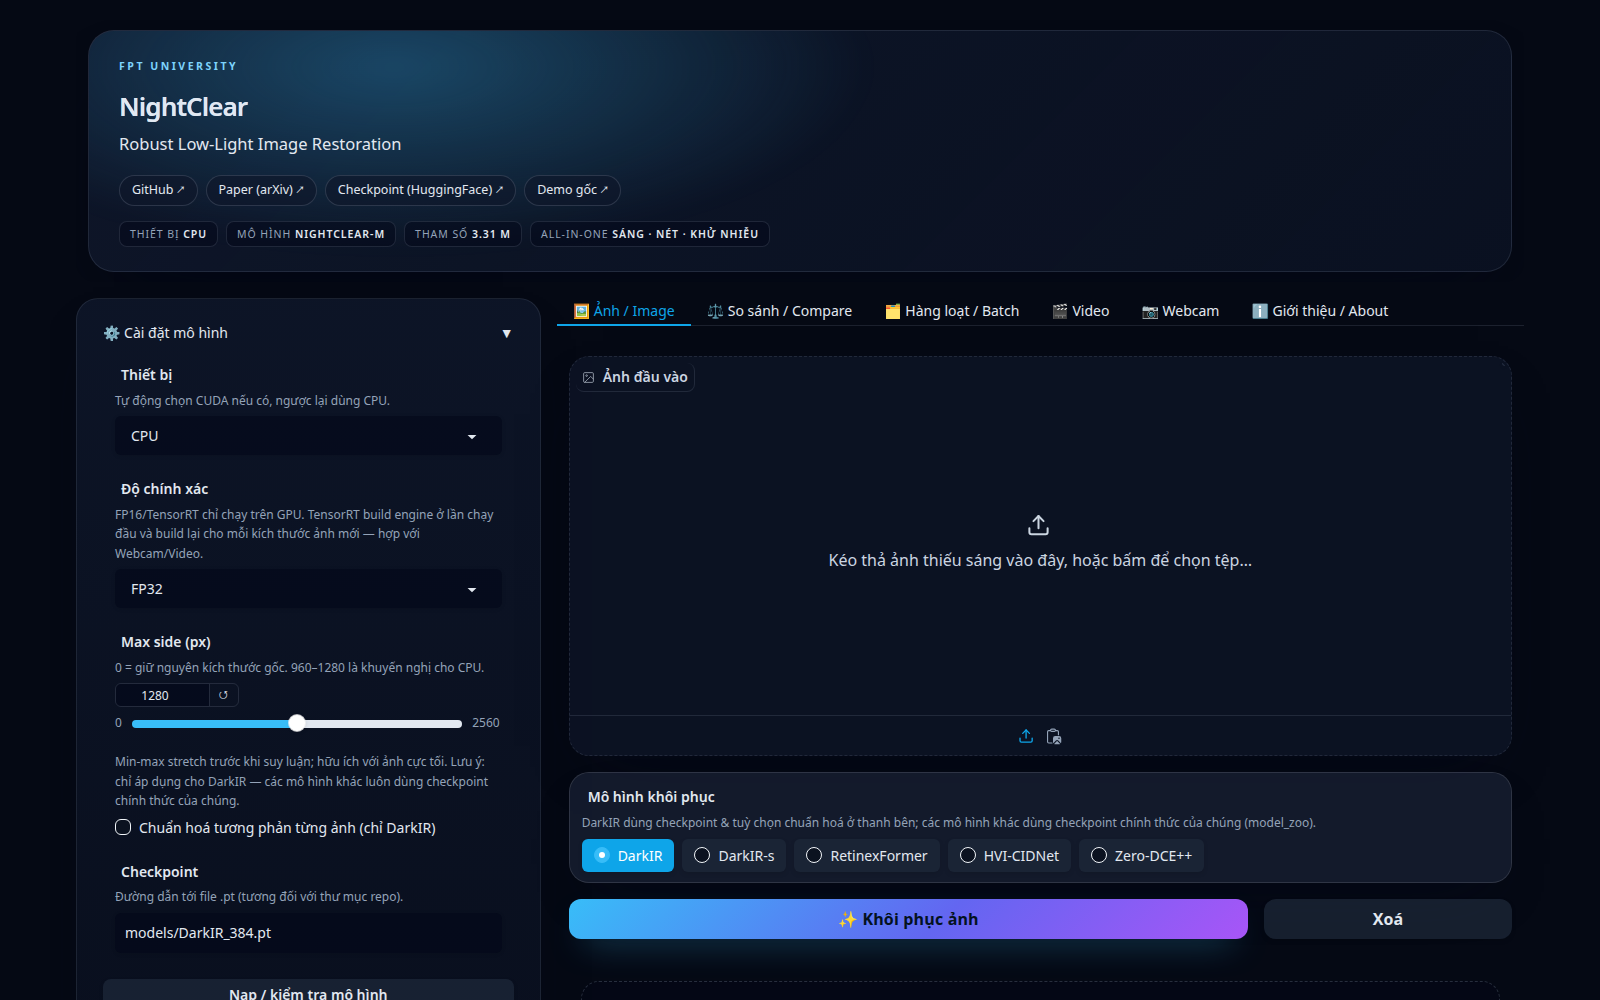
\includegraphics[width=\textwidth]{demo/ui.png}
        \end{column}
        \begin{column}{0.37\textwidth}
            \footnotesize
            \begin{itemize}
                \item \textbf{Tabs}: Image, Compare, Batch, Video, Webcam
                \item \textbf{5 models}: NightClear, NightClear-s, RetinexFormer, HVI-CIDNet, Zero-DCE++
                \item \textbf{Compare}: all models on one photo, ranked by speed
                \item \textbf{Precision}: FP32, FP16, TensorRT
                \item Runs on CPU or GPU, including free Google Colab
            \end{itemize}
        \end{column}
    \end{columns}
\end{frame}

% stat tile: big number + caption (defined outside the frame: frame bodies cannot hold #-parameters)
\newcommand{\stat}[2]{%
    \begin{beamercolorbox}[wd=\linewidth, ht=1.6cm, dp=0pt, center, rounded=true]{block body example}
        {\LARGE\bfseries\color{fptOrange} #1}\\[1mm]{\scriptsize #2}
    \end{beamercolorbox}}

\begin{frame}
    \frametitle{Practical Impact}

    \begin{columns}[t]
        \begin{column}{0.24\textwidth}\stat{+8.7 dB}{vs.\ best 2-model cascade}\end{column}
        \begin{column}{0.24\textwidth}\stat{5.3$\times$}{fewer MACs than LEDNet}\end{column}
        \begin{column}{0.24\textwidth}\stat{$-$55\%}{parameters vs.\ LEDNet}\end{column}
        \begin{column}{0.24\textwidth}\stat{3.31 M}{params, 13 MB, runs on CPU}\end{column}
    \end{columns}
    \vspace{2mm}
    \begin{columns}[t]
        \begin{column}{0.5\textwidth}
            \small
            \textbf{Value}
            \begin{itemize}
                \item One network instead of two to store, tune and run
                \item Fits laptops, edge and free cloud GPUs
                \item Handheld night shots without tripod or flash
            \end{itemize}
        \end{column}
        \begin{column}{0.5\textwidth}
            \small
            \textbf{Applications}
            \begin{itemize}
                \item Smartphone night mode
                \item Night surveillance / dash cams
                \item Pre-processing for detection in the dark (e.g.\ ExDark)
            \end{itemize}
        \end{column}
    \end{columns}
    {\tiny Numbers from paper Tables 1--2 (LOLBlur). The paper reports no runtime, so no time saving is claimed.}
\end{frame}
